% 2.0.SampleBuild.tex
%	Last update: 2021/03/15 F.Kanehori
\newpage
\section{サンプルプログラムのビルド}
\label{sec:SampleBuild}
\parindent=0pt

サンプルプログラムのビルド方法について説明します。

\bigskip
サンプルプログラムは、\SprTop{\core\src\Samples}以下に置かれています。
ここでは``BoxStack''を例にして説明します。

\bigskip
\SprTop{\core\src\Samples\Physics\BoxStack}に移動します。

適切なバージョンのソリューションファイル
\SlnFile{BoxStack}{nn.n}をVisual Studioで開き、
プロジェクト\tt{BodStack}をスタートアッププロジェクトに設定してビルドすれば
実行形式バイナリが生成されます。

\medskip
実行時にDLLが見つからないというエラーが発生した場合には、
\begin{center}\begin{tabular}{lcl}\hline
	32ビット環境のときは & --- & \SprTop{\dependency\bin\win32} \\\hline
	64ビット環境のときは & --- & \SprTop{\dependency\bin\win64} \\
				 & & \SprTop{\dependency\bin\win32} \\
				 & & の両方 \\\hline
\end{tabular} \end{center}
にパスを通してください。
Visual Studioから実行するときは、
プログラムのプロパティを開き、
[構成プロパティ]---[デバッグ]---[環境] に
``\,\tt{path=上記のパス}''とします。

\medskip
また、実行時に Assertion エラーが発生し
\begin{narrow}
``You have to define USE\_CLOSED\_SRC in SprDefs.h to use Spidar''
\end{narrow}
などと表示された場合には、
\SprTop{\core\include\SprUseClosedSrcOrNot.h}にある
\tt{\#undef}を \tt{\#define}と変更し、サンプルプログラムを再ビルドしてください。

\bigskip
\begin{narrow}[15pt]
	\begin{figure}[h]
	\begin{center}
	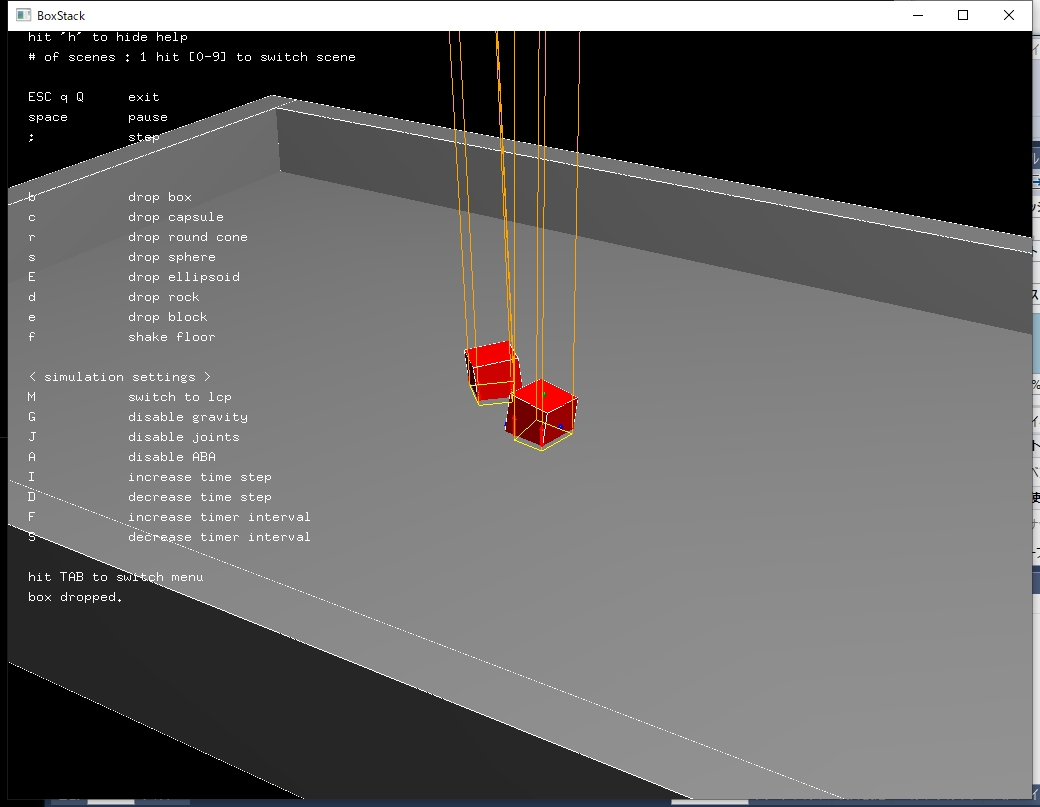
\includegraphics[width=0.5\textwidth]{fig/BoxStack_run.eps}
	\end{center}
	\caption{実行結果}
	\label{fig:BoxStack_run}
	\end{figure}
\end{narrow}


\bigskip
% end: 2.0.SampleBuild.tex
